\documentclass{beamer}

\usepackage[utf8]{inputenc}
\usepackage[T1]{fontenc}
\usepackage{color}
\usepackage{textcomp}
\usepackage{graphicx}

\usepackage{beamerthemesplit}
\usetheme{Berlin}
\useinnertheme{rounded}
\usecolortheme{dolphin}
\author{Valentin H\"anel}
\institute{Bernstein Center for Computational Neuroscience Berlin}

\title{Eine Git Einführung}
\definecolor{gray}{rgb}{0.10,0.10,0.10}
\date{April 2, 2009}

\begin{document}
%\frame{\titlepage}

\begin{frame}
	
\includegraphics[scale=0.05]{BCCN_logo_berlin.jpg}
	\titlepage
\end{frame}

\input{slides-01.tex}

\frame{
\frametitle{Zussamenhang}

\begin{figure}[ht]
	  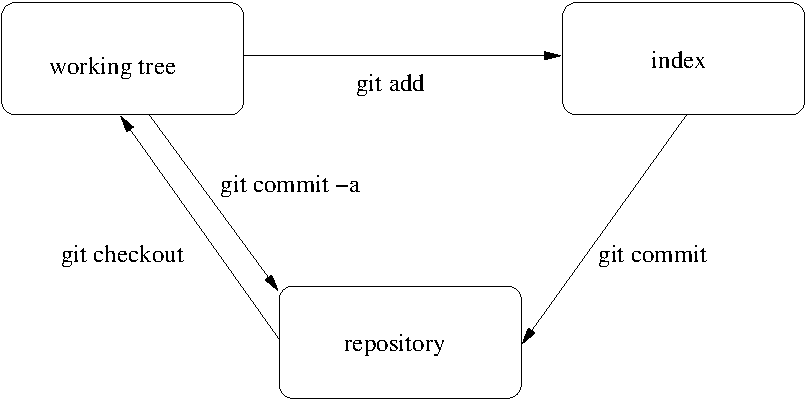
\includegraphics[scale=0.7]{git-im1.pdf}
      \caption{Zussamenhang von \textit{working tree}, \textit{index} und
      \textit{repository}}
\end{figure}
}

\input{slides-02.tex}

\frame{
\frametitle{Alternativen}

\begin{itemize}
    \item Meistens reicht f\"ur die Angabe von einem commit die ersten 4-7
        Zeichen des \textit{SHA-1 ID}
    \item @HEAD@ ist eine Referenz zu dem \textit{commit} der als
        \textit{parent} für den nächsten genommen wird, meist ist dies der
        neueste
    \item Relative Angaben werden mit \^{} und $\sim$ gemacht
    \item z.B. {\tt HEAD\^{}\^{}\^{}} und {\tt HEAD$\sim$3} sind equivalent und
        beschreiben beide den dritten \textit{commit} vor {\tt HEAD}
\end{itemize}

}

\input{slides-03.tex}

\section{.git}

\begin{frame}[fragile]
\frametitle{Inhalt von .git}

git speichert alles in dem Verzeichniss {\tt.git/} auch bekannt als \textbf{git
directory}

\begin{verbatim}
    % tree -L 1  .git/
    .
    |-- HEAD            # der gegenwärtige HEAD
    |-- config          # Konfiguration (user, email)
    |-- index           # der index
    |-- objects         # die eigentlichen Objekte

\end{verbatim}

\end{frame}


\end{document}
